\documentclass[t]{beamer}
\usetheme[deutsch]{KIT}
\setbeamercovered{transparent}
\setbeamertemplate{navigation symbols}{}

\KITfoot{Tutoriumsmaterial von Joachim Priesner, Sebastian Ullrich und Max Wagner \hspace{2.5cm} Basierend auf den Folien von Simon Stroh und Moritz v. Looz}
\usepackage[utf8]{inputenc}
\usepackage{amsmath}
\usepackage{ifthen}
\usepackage{amssymb}
\usepackage{tikz}
\usepackage{ngerman}
\usetikzlibrary{automata}
\usenavigationsymbols


\title{Theoretische Grundlagen der Informatik}
\subtitle{Tutorium}
\author{Moritz von Looz, Simon Stroh}

\institute[ITI]{Institut für Theoretische Informatik}

\TitleImage[height=\titleimageht]{images/tmaschine.png}

\newcommand{\N}{\ensuremath{\mathbb{N}}}
\newcommand{\M}{\ensuremath{\mathcal{M}}}
\newcommand{\classP}{\ensuremath{\mathcal{P}}}
\newcommand{\classNP}{\ensuremath{\mathcal{NP}}}
\newcommand{\co}{\ensuremath{\mathsf{co\text{-}}}}
\newcommand{\pot}{\ensuremath{\mathcal{P}}}
\newcommand{\abs}[1]{\ensuremath{\left\vert #1 \right\vert}}
\newcommand{\menge}[2]{\ensuremath{\left\lbrace #1 \,\middle\vert\, #2 \right\rbrace}}
\newcommand{\ducttape}[1]{\vspace{#1}}
\newcommand{\neglit}[1]{\overline{#1\vphantom{x^a}}}
\newcommand{\recipe}{\raisebox{-.3cm}{
\includegraphics[scale=.15]{images/chefs-cap.png}}\hspace{0.2cm}}

\newcommand{\invincible}{\setbeamercovered{invisible}} %  "Yesss! I am invincible!!" (Boris Grishenko)
\newcommand{\vincible}{\setbeamercovered{transparent}}

% \@ifundefined{tikzset}{}{\tikzset{initial text=}} % Text "start" bei Startknoten unterdrücken
\tikzstyle{every node}=[thick]
\tikzstyle{every line}=[thick]

\newcommand{\tutnr}[1]{
  \subtitle{Tutorium #1}
	\begin{frame}
		\maketitle
	\end{frame}
}

\newcommand{\uebnr}[1]{
  \subtitle{Anmerkungen zum #1. Übungsblatt}
	\begin{frame}
		\maketitle
	\end{frame}
}

\begin{document}

\tutnr{8}

%\begin{frame}
%\frametitle{Aufgabe}
%Jedes Jahr in der Vorweihnachtszeit steht die badische Hausfrau vor dem folgenden PLÄTZCHENDOSENPROBLEM (PDP):
%
%\hspace{1cm}\parbox{0.8\textwidth}{Das während der Adventszeit liebevoll hergestellte Weihnachtsgebäck soll bis zum Verzehr in Plätzchendosen gelagert werden.
%Es stehe eine bestimmte Anzahl gleichartiger Dosen mit einem gewissen Fassungsvermögen (Volumen) zur Verfügung, und es sei das Volumen jedes Plätzchens bekannt.
%
%Können die Plätzchen so auf die Dosen verteilt werden, dass bei allen Dosen der Deckel noch zugeht?}
%\begin{enumerate}
% \item Geben Sie eine formale Definition des PDP als Entscheidungsproblem an, wobei Sie der Einfachheit halber annehmen können, dass die Form der Plätzchen vernachlässigbar sei (es ist also lediglich verlangt, dass das Gesamtvolumen der Plätzchen in einer Dose deren Fassungsvermögen nicht überschreitet).
% \item Zeigen Sie die $\mathcal{NP}$-Vollständigkeit des PDP.
%\end{enumerate}
%\end{frame}

\section{Komplementsprachen}
\subsection{}

\begin{frame}
\frametitle{Komplementsprachen}
\begin{block}{Definition}
Zu einer Sprache $L \subseteq \Sigma^*$ definieren wir $\co L$ als das Komplement der Sprache, also
$\co L := \Sigma^*\setminus L$.
\end{block}
Für eine Klasse von Sprachen wie $\classP$ definieren wir die "`co"'-Klasse (wie z.B. $\co\classP$) als Menge der Komplemente (und nicht etwa als Komplement der Klasse).\\[8pt]
\pause
\textbf{Beispiel:} \co 3SAT: Die aussagenlogischen Formeln mit 3 Variablen pro Klausel, die nicht erfüllbar sind.\\[8pt]

\begin{block}{Anmerkungen}
\begin{itemize}
\item Ob $\mathcal{NP} = co-\mathcal{NP}$ ist eine offene Frage.
\item $\mathcal{NP} \neq co-\mathcal{NP}$ impliziert $\mathcal{P} \neq \mathcal{NP}$ 
\item Für $L \in \mathcal{NPC}$ gilt: $L \in co-\mathcal{NP} \iff \mathcal{NP} =  co-\mathcal{NP}$
\end{itemize}
\end{block}
\end{frame}

\begin{frame}
\frametitle{NPI}
\begin{block}{Definition}
$\mathcal{NP}\text{-Intermediate } (\mathcal{NPI}) := \mathcal{NP} \setminus (\mathcal{NPC} \cup \mathcal{P})$
\end{block}
$$ $$ % Yes, I am fully aware of the uglyness involved here

\begin{columns}%
		\begin{column}{0.6 \textwidth}%
			Da $\mathcal{NPI} \neq \emptyset \iff \mathcal{P} \neq \mathcal{NP}$, sind natürlich keine Probleme aus $\mathcal{NPI}$ bekannt, es gibt jedoch einige Kandidaten:
\begin{itemize}
	\item Graphisomorphie
	\item Faktorisieren
	\item Diskrete Logarithmen
	
\end{itemize}

Aufgrund ihrer Eigenschaften sind diese Probleme in der Kryptographie alle von großer Bedeutung.

		\end{column}%
		\begin{column}{0.35 \textwidth}%
	\ducttape{1cm} 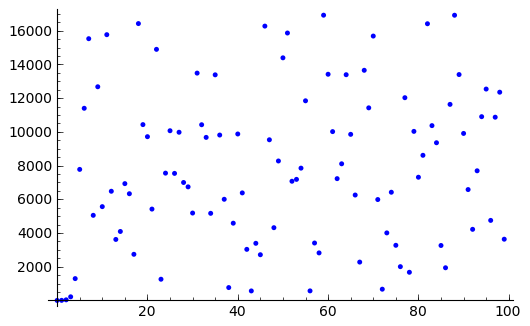
\includegraphics[scale=.3]{images/dlog.png}
		\end{column}%
	\end{columns}%
	\vfill%
\end{frame}


\begin{frame}
\frametitle{Aufgabe}
Betrachte das Problem NEAR TAUT: Gegeben sei ein Boolescher Ausdruck $A$. Es ist zu entscheiden, ob es höchstens eine Belegung der Variablen gibt, so dass $A$ falsch wird.
\begin{enumerate}
 \item Formuliere das komplementäre Problem co-NEAR TAUT.
 \item Zeige, dass NEAR TAUT in co-$\mathcal{NP}$ liegt.
\end{enumerate}
\end{frame}

\section{Pseudopolynomielle Algorithmen}
\subsection{aublvgskndrlgfvrnsawf}
%Pseudopolynomielle Algorithmen & Starke NP-Vollständigkeit
\begin{frame}
\frametitle{Pseudopolynomielle Algorithmen}
\begin{block}{Definition}
Ein Algorithmus wird \textbf{pseudopolyomiell} genannt, wenn seine Laufzeit polynomiell in der Eingabe \textit{bei Unärkodierung} ist.
\end{block}

$\Rightarrow$ Die Laufzeit hängt polynomiell von der Eingabelänge und der größten vorkommenden Zahl in der Eingabe ab. \micropause

Ein Problem heißt \textbf{schwach $\mathcal{NP}$-vollständig,} wenn es $\mathcal{NP}$-vollständig ist und ein pseudopolynomieller Algorithmus existiert, der das Problem entscheidet.\micropause
Existiert ein solcher Algorithmus nicht, so spricht man von einem \textbf{stark $\mathcal{NP}$-vollständigen} Problem.
\end{frame}

\begin{frame}
\frametitle{Aufgabe}
Das Entscheidungsproblem \textit{PRIMES} besteht darin, zu entscheiden, ob es sich bei einer gegebenen natürlichen Zahl $p>1$ um eine Primzahl handelt. 
Eine Probleminstanz von \textit{PRIMES} wird also durch eine natürliche Zahl kodiert.  \micropause
Ein naiver Algorithmus für \textit{PRIMES} könnte alle Zahlen $2,3,\ldots,p-1$ daraufhin überprüfen, ob sie die gegebene Zahl $p$ teilen.  \micropause
Zeige, dass dieser Algorithmus pseudopolynomiell ist. 
(Gib dazu eine Schranke für die Laufzeit an, die polynomiell in der Länge der Eingabe und der größten vorkommenden Zahl ist).
\end{frame}

\section{Such- und Aufzählungsprobleme}
\subsection{sdfsdofimlwegidrf}
%Suchprobleme, Aufzählungsprobleme
%NP-Schwere von Suchproblemen
%Integer Programming
\subsection{Suchprobleme}
\begin{frame}
 \frametitle{Suchprobleme}
 \begin{block}{Definition}
  Ein Suchproblem $\Pi$ wird beschrieben durch
  \begin{itemize}
   \item die Menge der Problembeispiele oder Instanzen $D_\Pi$
   \item für $I\in D_\Pi$ die Menge $S_\Pi(I)$ \emph{aller} Lösungen von $I$.
  \end{itemize}
 \end{block}
\begin{block}{Lösung}
 Die Lösung eines beliebigen Suchproblems für eine Instanz $D_\Pi$ ist
 \begin{itemize}
  \item ein beliebiges Element aus $S_\Pi(I)$, falls $S_\Pi(I) \not = \emptyset$
  \item $\emptyset$ sonst
 \end{itemize}
\end{block}
\end{frame}

\begin{frame}
\frametitle{Suchprobleme als Relationen}
Ein Suchproblem kann man auch als Relation auffassen, für $\Pi$ sei
$$ R_\Pi := \menge{ (x,s) }{ x \in D_\Pi, s\in S_\Pi(x)}$$
Eine Funktion $f: \Sigma^* \rightarrow \Sigma^*$ realisiert eine Relation $R$, wenn für alle $x \in \Sigma^*$ gilt:
$$f(x) = \begin{cases}
\epsilon, & \nexists y \in \Sigma^*\setminus\epsilon : (x,y) \in R\\
y, & \mbox{sonst, mit beliebigem }y:(x,y) \in R
\end{cases}$$
Eine Turingmaschine löst das durch $R_\Pi$ beschriebene Suchproblem $\Pi$, wenn sie eine Funktion berechnet, die $R_\Pi$ realisiert.
\end{frame}

\subsection{Orakelturingmaschinen}
\begin{frame}
\frametitle{Orakelturingmaschinen}
\begin{block}{Definition}

Eine Orakel-Turingmaschine $\mathcal{M}^G$ ist eine \textbf{deterministische} Turingmaschine, die ein zusätzliches Hilfsorakel enthält. \micropause

Dieses Hilfsorakel berechnet (zuverlässig!) in $\mathcal{O}(1)$ eine beliebige Funktion $G: \Sigma^* \rightarrow \Sigma^*$. \micropause

Zu jedem Zeitpunkt der Berechnung kann $\mathcal{M}$ Folgendes machen:
\begin{enumerate}
	\item Schreibe ein Wort $w$ auf ein spezielles "`Orakelband"'.
	\item Gehe über in einen Fragezustand $q_f$
	\item $\rightarrow$ Das Orakel schreibt in $\mathcal{O}(1)$ den Funktionswert $G(w)$ auf das Orakelband und $\M$ geht in den Antwortzustand $q_a$ über.
	\item Fahre mit der normalen Berechnung fort.
\end{enumerate} \ducttape{8pt}

\pause \textbf{Aufgabe:} Was hat dieses Hilfsorakel mit dem Orakel einer NTM zu tun? \solution{Gar nichts!}

%Eine Orakel-Turing-Maschine zum Orakel $G: \Sigma^* \rightarrow \Sigma^*$ ist eine Turingmaschine erweitert durch ein ausgezeichnetes Orakelband, sowie zwei zusätzlichen Zustände $q_f$ und $q_a$. Diese TM verhält sich für alle Zustände außer $q_f$ und $q_a$ wie eine normale TM.\\
%Kommt die Orakel-TM in den Zustand $q_f$, so wird der Inhalt des Orakelbandes von der Anfangsposition bis zur aktuellen Position des Kopfes auf dem Orakelband ersetzt durch seinen Funktionswert bzgl. $G$ und der Kopf an den Anfang des Orakelbandes zurückgesetzt.

\end{block}
\end{frame}

\begin{frame}
\frametitle{Beispiele}
Sei $\mathcal{P}^L$ die Klasse aller Entscheidungsprobleme, die in polynomieller Zeit von einer deterministischen Orakel-Turingmaschine mit Orakel für die charakteristische Funktion der Sprache $L$ entschieden werden können.\\
Dann ist
\begin{itemize}
\item $SAT \in \mathcal{P}^{SAT}$
\item $TSP \in \mathcal{P}^{SAT}$ 
\item $H_0 \in \mathcal{P}^{H_0}$
\end{itemize}
\end{frame}

%\begin{frame}
%\frametitle{Kurzer Exkurs}
%Einer der Hauptgründe, warum die $P \stackrel{?}{=} NP$ Frage so schwer ist, ist das bekannt ist, das es zwei Sprachen $A$ und $B$ gibt, für die gilt:
%\begin{enumerate}
%\item $\mathcal{P}^A = \mathcal{NP}^A$
%\item $\mathcal{P}^B \neq \mathcal{NP}^B$
%\end{enumerate}
%Ein Beweis für eine der beiden Aussagen darf also nicht mit Orakel weiterhin funktionieren.
%\end{frame}


\begin{frame}
\frametitle{Turingreduzierbarkeit}
\begin{block}{Definition}
Seien $R, R'$ Relationen über $\Sigma^*$. Eine Turing-Reduktion $\propto_T$ von $R$ auf $R'$, ist eine Orakel-Turing-Maschine $\mathcal{M}$
\begin{itemize}
\item deren Orakel die Relation $R'$ realisiert und
\item die selbst in polynomieller Zeit die Funktion $f$ berechnet, die $R$ realisiert. 
\end{itemize}
\end{block}
\end{frame}

\begin{frame}
 \frametitle{$\mathcal{NP}$-Schwere von Suchproblemen}
 \begin{block}{Definition}
  Ein Suchproblem $\Pi$ heißt $\mathcal{NP}$-schwer, falls es eine $\mathcal{NP}$-vollständige Sprache $L$ gibt mit $L \propto_T \Pi$.
 \end{block}
\end{frame}

\begin{frame}
 \frametitle{CLIQUE als Suchproblem}
 \begin{block}{Aufgabe}
  Formuliere CLIQUE als Suchproblem.
 \end{block}
 \solution{
 \begin{block}{CLIQUE-Suchproblem (Variante 2)}
  \begin{itemize}
   \item \textbf{Gegeben: } Graph $G = (V,E)$, Parameter $k\in \mathbb{N}$
   \item \textbf{Aufgabe: } Gib eine Clique in $G$ mit Kardinalität $k$ an, falls diese existiert.
  \end{itemize}
 \end{block}}
 \end{frame}
 
 \subsection{Aufzählungsprobleme}
\begin{frame}
 \frametitle{Aufzählungsprobleme}
 \begin{block}{Definition}
  Ein \emph{Aufzählungsproblem} $\Pi$ ist gegeben durch
  \begin{itemize}
   \item die Menge der Problembeispiele $D_\Pi$
   \item für $I \in D_\Pi$ die Menge $S_\Pi(I)$ aller Lösungen von $I$
  \end{itemize}
  \end{block}
  \begin{block}{Lösung}  
  Die \emph{Lösung} der Instanz $I$ eines Aufzählungsproblems $\Pi$ besteht in der Angabe der Kardinalität $|S_\Pi(I)|$ von $\Pi$.
 \end{block}
\end{frame}

 \begin{frame}
 \frametitle{CLIQUE als Aufzählungsproblem}
  \begin{block}{Aufgabe}
  Formuliere CLIQUE als Aufzählungsproblem.
\end{block}
\solution{
\begin{block}{CLIQUE-Aufzählungsproblem}
Eine Möglichkeit:
\begin{itemize}
 \item \textbf{Gegeben: } Graph $G = (V,E)$, Parameter $k\in \mathbb{N}$
 \item \textbf{Gesucht: } Anzahl der Cliquen in $G$ mit mindestens $k$ Knoten.
 \end{itemize}
\end{block}}
\end{frame}

\begin{frame}
	\frametitle{Aufgabe}
	
	\begin{enumerate}
		\item Zeige (informell): Aus $L \propto L'$ folgt, dass auch $L \propto_T L'$ gilt.
		\item Warum gilt nicht auch direkt die Umkehrung? Überlege dir dazu, dass gilt: $TSP \propto_T \co TSP$, aber $TSP \propto \co TSP$ ist schwer zu zeigen.
	\end{enumerate}
\end{frame}

\section{Integer Programming}
\subsection{asfasofiöogriödobkgffsawf}

\subsection{Integer Programming}
\begin{frame}
 \frametitle{INTEGER PROGRAMMING}
 \begin{block}{Definition (aus der Vorlesung)}
 \textbf{Gegeben: }
 \begin{itemize}
  \item $A = ((a_{ij})) \in \mathbb{Z}^{m \times n}$
  \item $b = (b_i) \in \mathbb{Z}^m, c = (c_j) \in \mathbb{Z}^n$
  \item $B\in \mathbb{Z}$
 \end{itemize}
\textbf{Frage: } Existieren $x_1, ..., x_n \in \mathbb{N}_0$, so dass gilt: $$\underbrace{\sum_{j=1}^n c_k \cdot x_j = B}_{\left\langle c, x\right\rangle = B}$$ $$\underbrace{\sum_{j=1}^n a_{ij} \cdot x_j \leq b_i}_{A \cdot x \leq b } \text{ für } 1 \leq i \leq m ?$$
 \end{block}
\end{frame}

\begin{frame}
 \frametitle{INTEGER PROGRAMMING}
 \begin{block}{Eigenschaften von INTEGER PROGRAMMING}
 \begin{itemize}
  \item INTEGER PROGRAMMING ist $\mathcal{NP}$-vollständig.
  \item Viele andere Probleme lassen sich leicht als INTEGER PROGRAMMING-Problem formulieren.
 \end{itemize}
 \end{block}
\end{frame}

\begin{frame}
\frametitle{Aufgabe}
Sei $G=(V, E)$ ein ungerichter Graph und $K \leq |V|$ eine natürliche Zahl. 
Ein \emph{Dominating Set} von $G$ ist eine Teilmenge $C \subseteq V$, so dass jeder Knoten $v$ entweder selbst in $C$ ist oder zu einem Knoten $w$ in $C$ adjazent ist. \micropause
Gibt es ein Dominating Set von $G$, das höchstens $k$ Knoten enthält?  \micropause

\begin{enumerate}
	\only<1>{\item Finde in folgendem Graphen ein möglichst kleines Dominating Set: \begin{center}
\includegraphics[scale=1.2]{images/tut7-graph}\end{center}}

\only<2>{\setcounter{enumi}{1}\item Formuliere DOMINATING SET als \emph{Integer Program}. }
\end{enumerate}
\end{frame}

\section{Schluss}
\subsection{assrögidlf}

\begin{frame}
	\frametitle{Bis zum nächsten Mal!}
	
	\begin{figure}[H]
		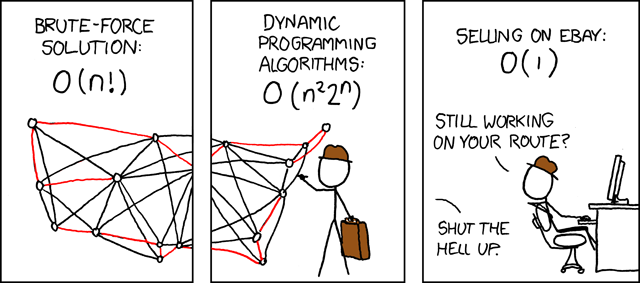
\includegraphics[width= \textwidth]{images/399_traveling_salesman}
		
		\textit{\scriptsize{What's the complexity class of the best linear programming cutting-plane techniques? I couldn't find it anywhere. Man, the Garfield guy doesn't have these problems $\ldots$}}
	\end{figure}
\end{frame}

\frame{
  \frametitle{Lizenzen}
  \center
  \includegraphics[width=2em]{images/by}
  \includegraphics[width=2em]{images/cc}
  \includegraphics[width=2em]{images/sa}
  \\
  {\tiny

Dieses Werk ist unter einem ``Creative Commons Namensnennung-Weitergabe unter gleichen Bedingungen 3.0 Deutschland``-Lizenzvertrag lizenziert. Um eine Kopie der Lizenz zu erhalten, gehen Sie bitte zu \href{http://creativecommons.org/licenses/by-sa/3.0/de/}{http://creativecommons.org/licenses/by-sa/3.0/de/} oder schreiben Sie an Creative Commons, 171 Second Street, Suite 300, San Francisco, California 94105, USA.\\
  \vspace{1cm}
  Davon ausgenommen sind das Titelbild, welches aus der März-April 2002 Ausgabe von American Scientist erschienen ist und ohne Erlaubnis verwendet wird, sowie das KIT Beamer Theme. Hierfür gelten die Bestimmungen der jeweiligen Urheber.
  \vspace{1cm}
  \\ 
  }
  %Habe hier die Reihenfolge etwas umgestellt, weil die Formatierung bei mir komisch aussah. 
  %Wenn es bei dir anders ist, kannst du es auch wieder zurückändern, dann haben wir unterschiedliche Kompilieroptionen
}

\end{document}
